\documentclass[11pt,a4paper]{article}

% ── Packages ──────────────────────────────────────────────────────────────────
\usepackage[utf8]{inputenc}
\usepackage[T1]{fontenc}
\usepackage{geometry}
\geometry{margin=2.5cm}
\usepackage{graphicx}
\usepackage{xcolor}
\usepackage{tikz}
\usetikzlibrary{arrows.meta, positioning, shapes.geometric, fit, calc, backgrounds, decorations.pathreplacing, patterns}
\usepackage{pgfplots}
\pgfplotsset{compat=1.18}
\usepackage{booktabs}
\usepackage{tabularx}
\usepackage{longtable}
\usepackage{enumitem}
\usepackage{listings}
\usepackage{hyperref}
\usepackage{fancyhdr}
\usepackage{titlesec}
\usepackage{amsmath}
\usepackage{fontawesome5}
\usepackage{tcolorbox}
\tcbuselibrary{skins, breakable}
\usepackage{float}
\usepackage{caption}
\usepackage{subcaption}
\usepackage{multicol}
\usepackage{pifont}

% ── Colours ───────────────────────────────────────────────────────────────────
\definecolor{substrate}{RGB}{30, 60, 114}
\definecolor{substratelt}{RGB}{70, 130, 200}
\definecolor{accent}{RGB}{220, 80, 60}
\definecolor{accentlt}{RGB}{255, 180, 140}
\definecolor{success}{RGB}{46, 139, 87}
\definecolor{warn}{RGB}{200, 150, 30}
\definecolor{codebg}{RGB}{245, 245, 250}
\definecolor{nodebg}{RGB}{230, 240, 255}
\definecolor{sensorbg}{RGB}{255, 235, 220}
\definecolor{motorbg}{RGB}{220, 255, 230}
\definecolor{modelbg}{RGB}{240, 230, 255}

% ── Listings ──────────────────────────────────────────────────────────────────
\lstset{
  language=Python,
  basicstyle=\ttfamily\small,
  keywordstyle=\color{substrate}\bfseries,
  stringstyle=\color{accent},
  commentstyle=\color{gray}\itshape,
  backgroundcolor=\color{codebg},
  frame=single,
  rulecolor=\color{substrate!30},
  breaklines=true,
  showstringspaces=false,
  tabsize=4,
  xleftmargin=1em,
  framexleftmargin=0.5em,
  numbers=left,
  numberstyle=\tiny\color{gray},
  numbersep=8pt,
}

% ── Header / Footer ──────────────────────────────────────────────────────────
\pagestyle{fancy}
\fancyhf{}
\fancyhead[L]{\small\textcolor{substrate}{\textbf{Substrate House}}}
\fancyhead[R]{\small\textcolor{substrate}{Neurobehavioural Adaptive Robot}}
\fancyfoot[C]{\thepage}
\renewcommand{\headrulewidth}{0.4pt}
\renewcommand{\headrule}{\hbox to\headwidth{\color{substrate}\leaders\hrule height \headrulewidth\hfill}}

% ── Section Styling ───────────────────────────────────────────────────────────
\titleformat{\section}
  {\Large\bfseries\color{substrate}}
  {\thesection}{1em}{}[\vspace{-0.5em}\textcolor{substrate}{\rule{\textwidth}{0.4pt}}]
\titleformat{\subsection}
  {\large\bfseries\color{substrate!80}}
  {\thesubsection}{1em}{}

% ── Custom Boxes ──────────────────────────────────────────────────────────────
\newtcolorbox{riskbox}[1][]{
  colback=accent!5, colframe=accent!70, title={\faExclamationTriangle\; Risk}, fonttitle=\bfseries, #1
}
\newtcolorbox{notebox}[1][]{
  colback=substrate!5, colframe=substrate!50, title={\faInfoCircle\; Note}, fonttitle=\bfseries, #1
}
\newtcolorbox{milestonebox}[1][]{
  colback=success!5, colframe=success!70, fonttitle=\bfseries, #1
}

% ── Title ─────────────────────────────────────────────────────────────────────
\title{%
  \vspace{-1cm}
  \textcolor{substrate}{\rule{\textwidth}{1.5pt}}\\[0.6cm]
  {\Huge\bfseries\textcolor{substrate}{Neurobehavioural Adaptive Robot}}\\[0.3cm]
  {\Large\textcolor{substrate!70}{Complete Build Plan for a Biosignal-Driven\\Interactive Robot Platform}}\\[0.4cm]
  \textcolor{substrate}{\rule{\textwidth}{1.5pt}}
}
\author{%
  \textbf{Substrate House}\\
  \textit{Neuroscience \textperiodcentered\ Engineering \textperiodcentered\ Data Science}\\
  London, UK
}
\date{April 2026 \textperiodcentered\ v1.0}

% ══════════════════════════════════════════════════════════════════════════════
\begin{document}
\maketitle
\thispagestyle{fancy}

% ── Abstract ──────────────────────────────────────────────────────────────────
\begin{abstract}
\noindent
This document presents a complete build plan for a physically embodied robot that reads real-time multimodal biosignal data from a human participant, passes it through a neurobehavioural foundation model, and adapts its behaviour based on the inferred cognitive and physiological state. The plan covers robot form factor, hardware components, compute architecture, software stack, real-time data pipeline, behaviour design, and a phased build schedule with milestones. The target is a working prototype within 14 weeks.
\end{abstract}

\tableofcontents
\newpage

% ══════════════════════════════════════════════════════════════════════════════
\section{System Overview}
\label{sec:overview}

The system consists of three principal subsystems: (1)~wearable biosignal sensors on the human, (2)~an edge compute unit running the foundation model, and (3)~a physically embodied robot that adapts its behaviour in real time. Figure~\ref{fig:system-overview} shows the high-level architecture.

\begin{figure}[H]
\centering
\begin{tikzpicture}[
    >=Stealth,
    node distance=1.5cm,
    block/.style={rectangle, rounded corners=6pt, draw=#1!70, fill=#1!10, text width=4.2cm, minimum height=1.8cm, align=center, font=\small\bfseries, line width=1pt},
    dataflow/.style={->, thick, color=substrate!70},
    label/.style={font=\scriptsize\itshape, text=gray}
  ]

  % Human
  \node[block=accent] (human) {
    \faUser\ \textcolor{accent!80}{Human Participant}\\[3pt]
    \footnotesize\normalfont EEG \textperiodcentered\ Eye Tracking\\
    \footnotesize\normalfont fNIRS \textperiodcentered\ StretchSense\\
    \footnotesize\normalfont Microphone
  };

  % Compute
  \node[block=substrate, right=2.5cm of human] (compute) {
    \faMicrochip\ \textcolor{substrate!80}{Edge Compute}\\[3pt]
    \footnotesize\normalfont Jetson Orin NX\\
    \footnotesize\normalfont Foundation Model\\
    \footnotesize\normalfont Behaviour Policy
  };

  % Robot
  \node[block=success, right=2.5cm of compute] (robot) {
    \faRobot\ \textcolor{success!80}{Robot Platform}\\[3pt]
    \footnotesize\normalfont Mobile Base\\
    \footnotesize\normalfont Expressive Head\\
    \footnotesize\normalfont LEDs \textperiodcentered\ Speaker
  };

  % Arrows
  \draw[dataflow] (human.east) -- node[above, label] {LSL / WiFi} node[below, label] {biosignal streams} (compute.west);
  \draw[dataflow] (compute.east) -- node[above, label] {ROS2 / USB} node[below, label] {motor commands} (robot.west);
  \draw[dataflow, dashed, accent!50] (robot.south) -- ++(0,-1) -| node[below, pos=0.25, label] {physical interaction \& proximity} (human.south);

  % Title
  \node[above=0.8cm of compute, font=\footnotesize\bfseries\color{substrate}] {NEUROBEHAVIOURAL ADAPTIVE ROBOT SYSTEM};

\end{tikzpicture}
\caption{High-level system architecture. Biosignal data flows from the human through edge compute to the robot; the robot's physical behaviour feeds back to the human through the interaction loop.}
\label{fig:system-overview}
\end{figure}


% ══════════════════════════════════════════════════════════════════════════════
\section{Robot Form Factor and Design Rationale}
\label{sec:form-factor}

\subsection{Recommended Form: Mobile Tabletop Companion}

The primary output channel is \textbf{behavioural adaptation}---pace, proximity, expression, movement style---not physical manipulation. This dictates a mobile companion form factor rather than an arm or humanoid.

\begin{figure}[H]
\centering
\begin{tikzpicture}[scale=1.0]
  % Base platform
  \fill[substrate!15, rounded corners=4pt] (-2.5, 0) rectangle (2.5, 1.2);
  \draw[substrate!50, rounded corners=4pt, thick] (-2.5, 0) rectangle (2.5, 1.2);

  % Wheels
  \foreach \x in {-2.0, -0.7, 0.7, 2.0} {
    \fill[substrate!60, rounded corners=2pt] (\x-0.25, -0.15) rectangle (\x+0.25, 0.15);
  }

  % Body column
  \fill[substrate!10, rounded corners=3pt] (-1.2, 1.2) rectangle (1.2, 3.0);
  \draw[substrate!40, rounded corners=3pt, thick] (-1.2, 1.2) rectangle (1.2, 3.0);

  % Jetson label
  \node[font=\tiny, text=substrate!70] at (0, 2.1) {Jetson Orin NX};
  \node[font=\tiny, text=substrate!70] at (0, 1.7) {+ Teensy 4.1};

  % Neck (pan-tilt)
  \draw[substrate!50, thick] (-0.15, 3.0) -- (-0.15, 3.5);
  \draw[substrate!50, thick] (0.15, 3.0) -- (0.15, 3.5);
  \fill[warn!50, circle] (0, 3.25) circle (0.12);
  \node[font=\tiny, text=warn!80, right] at (0.3, 3.25) {pan-tilt};

  % Head
  \fill[substratelt!20, rounded corners=8pt] (-1.5, 3.5) rectangle (1.5, 5.5);
  \draw[substratelt!60, rounded corners=8pt, thick] (-1.5, 3.5) rectangle (1.5, 5.5);

  % Face display (round)
  \fill[white] (0, 4.5) circle (0.9);
  \draw[substrate!30, thick] (0, 4.5) circle (0.9);

  % Eyes
  \fill[substrate] (-0.35, 4.65) ellipse (0.22 and 0.15);
  \fill[substrate] (0.35, 4.65) ellipse (0.22 and 0.15);
  % Eye highlights
  \fill[white] (-0.28, 4.7) circle (0.06);
  \fill[white] (0.42, 4.7) circle (0.06);
  % Mouth
  \draw[substrate, thick, line cap=round] (-0.25, 4.15) .. controls (0, 4.0) .. (0.25, 4.15);

  % LED ring
  \foreach \a in {0,30,...,330} {
    \fill[accent!60] (0, 4.5) ++(\a:1.05) circle (0.06);
  }

  % Speaker
  \fill[gray!30, rounded corners=2pt] (-0.4, 3.65) rectangle (0.4, 3.85);
  \node[font=\tiny, text=gray] at (0, 3.75) {\faVolumeUp};

  % Dimension annotations
  \draw[<->, gray, thin] (-3.2, 0) -- node[left, font=\tiny, text=gray] {$\sim$45cm} (-3.2, 5.5);
  \draw[<->, gray, thin] (-2.5, -0.5) -- node[below, font=\tiny, text=gray] {$\sim$30cm} (2.5, -0.5);

  % Labels
  \node[font=\scriptsize\bfseries, text=substrate, right] at (2.8, 4.5) {Expressive Head};
  \draw[->, substrate!40, thin] (2.8, 4.5) -- (1.6, 4.5);

  \node[font=\scriptsize\bfseries, text=substrate, right] at (2.8, 2.1) {Compute Bay};
  \draw[->, substrate!40, thin] (2.8, 2.1) -- (1.3, 2.1);

  \node[font=\scriptsize\bfseries, text=substrate, right] at (2.8, 0.6) {Mobile Base};
  \draw[->, substrate!40, thin] (2.8, 0.6) -- (2.6, 0.6);

  \node[font=\scriptsize\bfseries, text=accent, left] at (-2.8, 4.5) {LED Ring};
  \draw[->, accent!40, thin] (-2.8, 4.5) -- (-1.6, 4.5);

  \node[font=\scriptsize\bfseries, text=warn, left] at (-2.8, 3.25) {Pan-Tilt};
  \draw[->, warn!40, thin] (-2.8, 3.25) -- (-0.3, 3.25);

\end{tikzpicture}
\caption{Robot form factor concept. A mobile base supports a compute bay and an expressive pan-tilt head with round display face, LED ring, and speaker. Total height approximately 45\,cm.}
\label{fig:robot-form}
\end{figure}

\subsection{Design Rationale}

\begin{itemize}[leftmargin=1.5em]
  \item \textbf{Mobile base} enables proximity modulation---the robot can approach or retreat based on arousal and stress levels.
  \item \textbf{Expressive head} with pan-tilt provides the fastest, most legible feedback channel: gaze direction, expression changes, and head orientation communicate social signals that humans read instinctively.
  \item \textbf{Compact tabletop scale} ($\sim$30--50\,cm) keeps the build mechanically simple and safe for close interaction.
  \item \textbf{No arms in v1}---manipulation adds 10$\times$ complexity with minimal benefit for adaptive behaviour output.
\end{itemize}


% ══════════════════════════════════════════════════════════════════════════════
\section{Hardware Specification}
\label{sec:hardware}

\subsection{Compute Hardware}

\begin{table}[H]
\centering
\caption{Compute components.}
\label{tab:compute}
\begin{tabularx}{\textwidth}{lllX}
\toprule
\textbf{Component} & \textbf{Part} & \textbf{Cost (£)} & \textbf{Role} \\
\midrule
Edge AI Computer & NVIDIA Jetson Orin NX 16\,GB & 450--550 & Foundation model inference (PyTorch, TensorRT, $\sim$100 TOPS INT8) \\
Carrier Board & Seeed reComputer J4012 & incl. & Jetson carrier with I/O breakout \\
Microcontroller & Teensy 4.1 (600\,MHz Cortex-M7) & 25 & Real-time motor control, sensor polling, safety watchdog \\
Offload Server (opt.) & Linux PC + RTX 4090 & varies & If model exceeds Jetson capacity \\
\bottomrule
\end{tabularx}
\end{table}

\subsection{Mobile Base}

\begin{table}[H]
\centering
\caption{Mobile base options.}
\label{tab:base}
\begin{tabularx}{\textwidth}{llX}
\toprule
\textbf{Component} & \textbf{Part} & \textbf{Notes} \\
\midrule
Base Platform & Robotis TurtleBot4 Lite (£1,100) & ROS2-native out of box; saves 2--3 months vs custom \\
Alt: Custom Chassis & Aluminium 4WD ($\sim$30$\times$25\,cm) & Cheaper but requires more integration \\
Alt: Motors & 4$\times$ JGB37-520 DC geared (12\,V, encoders) & Encoders essential for odometry \\
Motor Driver & Cytron MDD10A dual H-bridge & Simple, reliable \\
Robot IMU & BNO055 9-DOF & Robot orientation and acceleration \\
LiDAR (v2) & RPLidar A1M8 & SLAM and navigation \\
\bottomrule
\end{tabularx}
\end{table}

\subsection{Expressive Head}

\begin{table}[H]
\centering
\caption{Head and expression components.}
\label{tab:head}
\begin{tabularx}{\textwidth}{llX}
\toprule
\textbf{Component} & \textbf{Part} & \textbf{Notes} \\
\midrule
Pan-Tilt Servos & Dynamixel XL330-M288-T ($\times$2) & Excellent small servos; Dynamixel SDK has ROS2 support \\
Servo Controller & Dynamixel U2D2 & USB-to-Dynamixel interface \\
Face Display & Waveshare 5'' round LCD & Renders animated eyes and expressions \\
Speaker & 3\,W speaker + MAX98357A I2S amp & Tones, simple vocalisations \\
LED Ring & NeoPixel WS2812B (24-LED) & Ambient state indicator \\
Housing & 3D-printed PLA/PETG & Custom head shell \\
\bottomrule
\end{tabularx}
\end{table}

\subsection{Biosignal Acquisition (Wearable on Human)}

\begin{table}[H]
\centering
\caption{Biosignal hardware and streaming protocols.}
\label{tab:biosignal}
\begin{tabularx}{\textwidth}{llX}
\toprule
\textbf{Stream} & \textbf{Hardware} & \textbf{Protocol} \\
\midrule
EEG & mBrainTrain Smarting PRO (24\,ch) \textit{or} OpenBCI Cyton+Daisy (16\,ch) & LSL (native) \\
Eye Tracking & Pupil Labs Neon \textit{or} Tobii Pro Glasses 3 & LSL (plugin) \\
fNIRS & NIRx NIRSport2 (wireless) & LSL (native) \\
StretchSense & Existing StretchSense gloves & Custom UDP $\rightarrow$ LSL relay \\
Microphone & Rode Wireless GO II & ALSA $\rightarrow$ LSL \\
Screen Recording & OBS Studio + NDI & LSL timestamp markers \\
\bottomrule
\end{tabularx}
\end{table}

\subsection{Power System}

\begin{table}[H]
\centering
\caption{Power components.}
\label{tab:power}
\begin{tabularx}{\textwidth}{lX}
\toprule
\textbf{Component} & \textbf{Specification} \\
\midrule
Robot Battery & 12\,V 5\,Ah LiPo (motors and base) \\
Jetson Power & 7--20\,V input, $\sim$15\,W typical / 25\,W peak; Pololu 12\,V-to-19\,V step-up from robot battery \\
Battery Management & Low-voltage cutoff; monitored via Teensy ADC \\
\bottomrule
\end{tabularx}
\end{table}

\subsection{Cost Summary}

\begin{table}[H]
\centering
\caption{Estimated total cost (excluding biosignal hardware already owned).}
\label{tab:cost}
\begin{tabular}{lr}
\toprule
\textbf{Item} & \textbf{Est. Cost (£)} \\
\midrule
Jetson Orin NX 16\,GB + carrier board & 550 \\
TurtleBot4 Lite & 1,100 \\
Dynamixel XL330-M288-T ($\times$2) + U2D2 & 120 \\
Waveshare 5'' round display & 45 \\
NeoPixel 24-LED ring & 10 \\
Speaker + MAX98357A amp & 15 \\
Teensy 4.1 & 25 \\
12\,V LiPo battery + charger & 80 \\
DC-DC converter (Pololu) & 15 \\
3D printing filament & 30 \\
Cables, connectors, misc & 50 \\
\midrule
\textbf{Total} & \textbf{$\sim$£2,040} \\
\bottomrule
\end{tabular}
\end{table}


% ══════════════════════════════════════════════════════════════════════════════
\section{Compute Architecture}
\label{sec:compute}

\subsection{Architecture Diagram}

Figure~\ref{fig:compute-arch} shows the full compute pipeline from biosignal acquisition through model inference to motor command generation.

\begin{figure}[H]
\centering
\begin{tikzpicture}[
    >=Stealth,
    node distance=0.8cm,
    every node/.style={font=\small},
    proc/.style={rectangle, rounded corners=4pt, draw=#1!60, fill=#1!8, minimum width=5cm, minimum height=1.1cm, align=center, line width=0.8pt},
    hw/.style={rectangle, rounded corners=4pt, draw=#1!60, fill=#1!15, minimum width=5cm, minimum height=1.1cm, align=center, line width=0.8pt, font=\small\bfseries},
    arrow/.style={->, thick, substrate!60},
    lbl/.style={font=\scriptsize\itshape, text=gray}
  ]

  % Left column: Human + Sensors
  \node[hw=accent] (sensors) {\faUser\ Human Wearable Sensors};
  \node[below=0.3cm of sensors, font=\scriptsize, text=gray] (slist) {EEG \textperiodcentered\ Eye Tracking \textperiodcentered\ fNIRS \textperiodcentered\ StretchSense \textperiodcentered\ Mic};

  % Jetson column
  \node[proc=substratelt, below=1.2cm of slist] (lsl) {LSL Receiver Node};
  \node[proc=substratelt, below=0.6cm of lsl] (preproc) {Preprocessing Node};
  \node[below=0.1cm of preproc, font=\scriptsize, text=gray] (pplist) {Bandpass \textperiodcentered\ Artifact Rej. \textperiodcentered\ Windowing \textperiodcentered\ Alignment};
  \node[proc=violet, below=0.8cm of pplist] (model) {\faBrain\ Foundation Model Inference};
  \node[below=0.1cm of model, font=\scriptsize, text=gray] (mlist) {TensorRT / ONNX Runtime on Jetson GPU};
  \node[proc=substratelt, below=0.8cm of mlist] (policy) {Behaviour Policy Node};
  \node[below=0.1cm of policy, font=\scriptsize, text=gray] (plist) {State Vector $\rightarrow$ Action Commands};

  % Robot hardware
  \node[hw=success, below=1.0cm of plist] (teensy) {\faMicrochip\ Teensy 4.1 (Real-Time Control)};
  \node[hw=success, below=0.6cm of teensy] (actuators) {\faRobot\ Motors \textperiodcentered\ Servos \textperiodcentered\ LEDs \textperiodcentered\ Speaker};

  % Arrows
  \draw[arrow] (sensors.south) -- node[right, lbl] {WiFi / LSL} (lsl.north);
  \draw[arrow] (lsl.south) -- node[right, lbl] {ROS2 topics} (preproc.north);
  \draw[arrow] (preproc.south) -- ++(0,-0.55) -- (model.north);
  \draw[arrow] (model.south) -- ++(0,-0.55) -- node[right, lbl, pos=0.2] {state vector} (policy.north);
  \draw[arrow] (policy.south) -- ++(0,-0.65) -- node[right, lbl, pos=0.2] {/cmd\_vel, /head\_pose, /led, ...} (teensy.north);
  \draw[arrow] (teensy.south) -- node[right, lbl] {PWM / Serial} (actuators.north);

  % Jetson boundary
  \begin{scope}[on background layer]
    \node[fit=(lsl)(preproc)(pplist)(model)(mlist)(policy)(plist), inner sep=12pt, draw=substrate!40, dashed, rounded corners=8pt, fill=substrate!3, label={[font=\footnotesize\bfseries\color{substrate}]above:Jetson Orin NX (ROS2 + PyTorch)}] {};
  \end{scope}

  % Optional offload
  \node[proc=gray, right=2.2cm of model] (server) {Offload Server\\(if model too large)};
  \draw[->, dashed, gray, thick] (model.east) -- node[above, lbl] {gRPC / WiFi} (server.west);

\end{tikzpicture}
\caption{Compute architecture. All ROS2 nodes run on the Jetson Orin NX. The Teensy handles hard real-time motor control. An optional offload server handles inference if the model exceeds Jetson capacity.}
\label{fig:compute-arch}
\end{figure}

\subsection{Model Optimisation for Edge Deployment}

The foundation model must run inference in \textbf{$<$200\,ms per window} to feel responsive:

\begin{enumerate}[leftmargin=1.5em]
  \item \textbf{Export to ONNX}, then optimise with \textbf{TensorRT} on Jetson---expect 2--5$\times$ speedup over vanilla PyTorch.
  \item \textbf{Quantise to FP16 or INT8}. For biosignal embeddings, FP16 is almost always lossless.
  \item If the model exceeds $\sim$500M parameters, \textbf{offload to a server} over WiFi. Budget $\sim$20--50\,ms network round-trip on local 5\,GHz WiFi.
  \item Target: \textbf{5--10\,Hz inference rate} (100--200\,ms per cycle).
\end{enumerate}

\begin{notebox}
Design the inference node to support both local and remote execution from day one. A simple configuration flag can switch between \texttt{LocalInferenceBackend} and \texttt{RemoteInferenceBackend} (gRPC client).
\end{notebox}


% ══════════════════════════════════════════════════════════════════════════════
\section{Software and Programming Stack}
\label{sec:software}

\subsection{Stack Overview}

\begin{figure}[H]
\centering
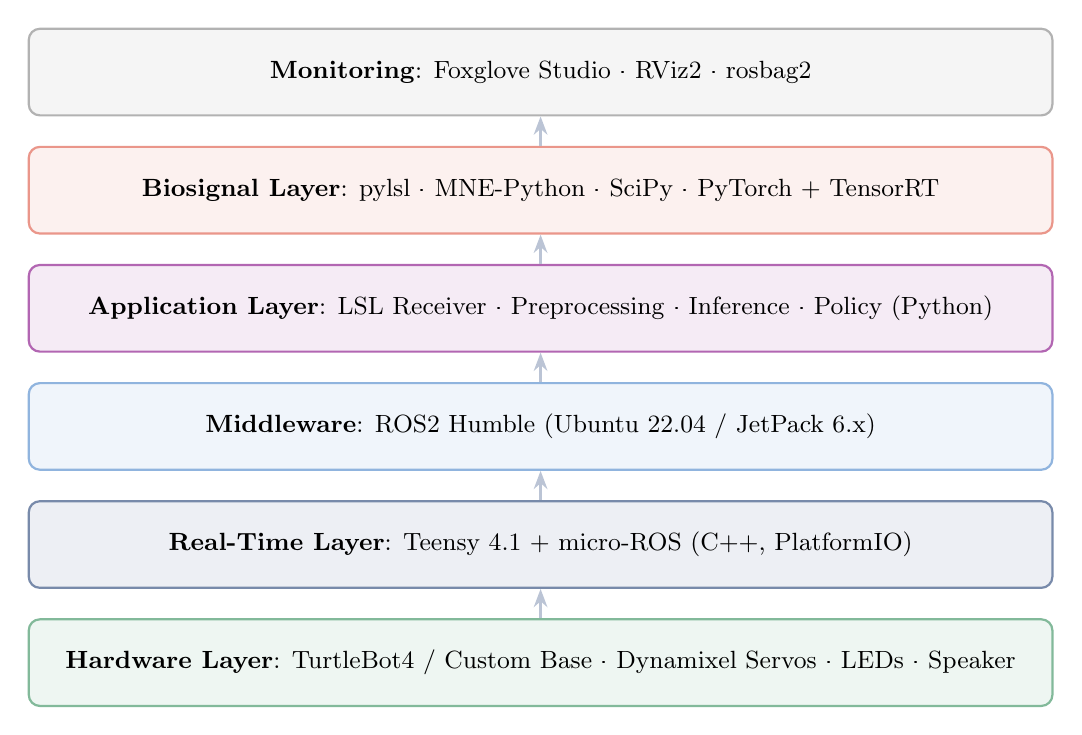
\begin{tikzpicture}[
    layer/.style={rectangle, rounded corners=4pt, minimum width=13cm, minimum height=1.1cm, align=center, font=\small, line width=0.8pt},
    >=Stealth
  ]

  \node[layer, draw=success!60, fill=success!8] (hw) at (0, 0) {\textbf{Hardware Layer}: TurtleBot4 / Custom Base \textperiodcentered\ Dynamixel Servos \textperiodcentered\ LEDs \textperiodcentered\ Speaker};
  \node[layer, draw=substrate!60, fill=substrate!8] (rt) at (0, 1.5) {\textbf{Real-Time Layer}: Teensy 4.1 + micro-ROS (C++, PlatformIO)};
  \node[layer, draw=substratelt!60, fill=substratelt!8] (mid) at (0, 3.0) {\textbf{Middleware}: ROS2 Humble (Ubuntu 22.04 / JetPack 6.x)};
  \node[layer, draw=violet!60, fill=violet!8] (app) at (0, 4.5) {\textbf{Application Layer}: LSL Receiver \textperiodcentered\ Preprocessing \textperiodcentered\ Inference \textperiodcentered\ Policy (Python)};
  \node[layer, draw=accent!60, fill=accent!8] (bio) at (0, 6.0) {\textbf{Biosignal Layer}: pylsl \textperiodcentered\ MNE-Python \textperiodcentered\ SciPy \textperiodcentered\ PyTorch + TensorRT};
  \node[layer, draw=gray!60, fill=gray!8] (mon) at (0, 7.5) {\textbf{Monitoring}: Foxglove Studio \textperiodcentered\ RViz2 \textperiodcentered\ rosbag2};

  \foreach \a/\b in {hw/rt, rt/mid, mid/app, app/bio, bio/mon} {
    \draw[->, substrate!30, thick] (\a.north) -- (\b.south);
  }

\end{tikzpicture}
\caption{Software stack layers from hardware to monitoring.}
\label{fig:software-stack}
\end{figure}

\subsection{Key Libraries}

\begin{table}[H]
\centering
\caption{Software libraries by purpose.}
\label{tab:libraries}
\begin{tabularx}{\textwidth}{lX}
\toprule
\textbf{Purpose} & \textbf{Library} \\
\midrule
Biosignal streaming & \texttt{pylsl} (Lab Streaming Layer Python bindings) \\
EEG preprocessing & \texttt{MNE-Python} (filtering, artifact rejection, epoching) \\
Signal processing & \texttt{SciPy} (bandpass filters, spectral analysis) \\
Model inference & \texttt{PyTorch} + \texttt{torch2trt} or \texttt{onnxruntime-gpu} \\
Behaviour policy & Custom Python; later \texttt{Gymnasium} for RL \\
Robot control & \texttt{rclpy} (ROS2 Python), \texttt{geometry\_msgs}, \texttt{Dynamixel SDK} \\
Teensy firmware & \texttt{micro-ROS} Arduino library, \texttt{Dynamixel2Arduino} \\
Orchestration & ROS2 Launch (Python launch files) \\
Logging & \texttt{rosbag2} for recording all ROS2 topics \\
Visualisation & \texttt{RViz2}, \texttt{Foxglove Studio} (web-based) \\
\bottomrule
\end{tabularx}
\end{table}

\subsection{ROS2 Node Architecture}

\begin{figure}[H]
\centering
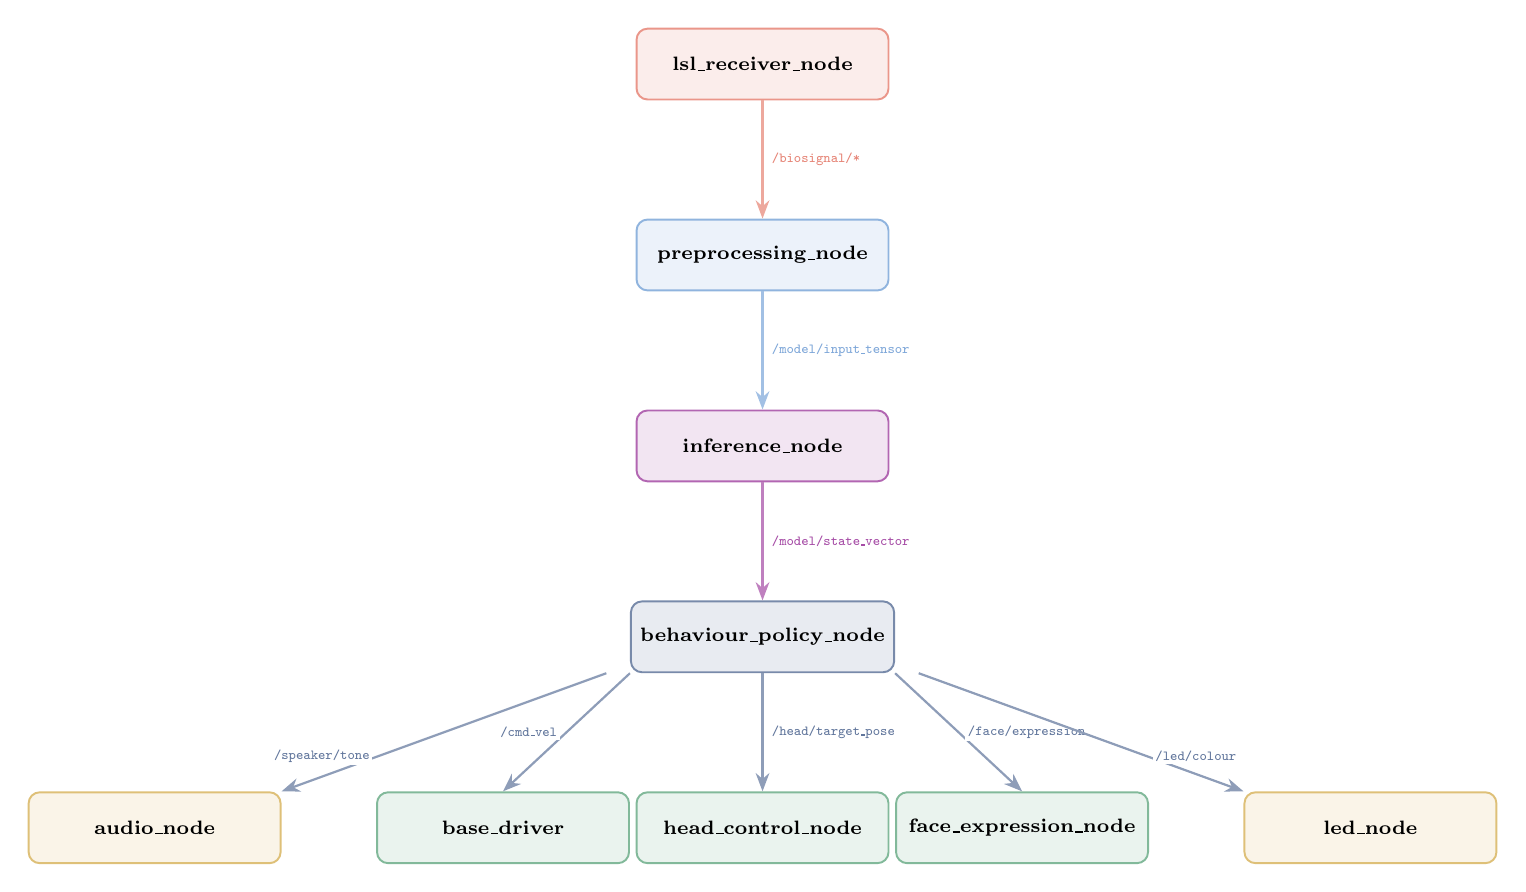
\begin{tikzpicture}[
    >=Stealth,
    node distance=0.6cm and 1.8cm,
    rosnode/.style={rectangle, rounded corners=4pt, draw=#1!60, fill=#1!10, minimum width=3.2cm, minimum height=0.9cm, align=center, font=\scriptsize\bfseries, line width=0.7pt},
    topic/.style={->, thick, #1!50, font=\tiny\ttfamily},
    topicname/.style={font=\tiny\ttfamily, text=#1!70, fill=white, inner sep=1pt}
  ]

  % Nodes
  \node[rosnode=accent] (lsl) {lsl\_receiver\_node};
  \node[rosnode=substratelt, below=1.5cm of lsl] (preproc) {preprocessing\_node};
  \node[rosnode=violet, below=1.5cm of preproc] (infer) {inference\_node};
  \node[rosnode=substrate, below=1.5cm of infer] (policy) {behaviour\_policy\_node};

  % Output nodes
  \node[rosnode=success, below left=1.5cm and 0cm of policy] (base) {base\_driver};
  \node[rosnode=success, below=1.5cm of policy] (head) {head\_control\_node};
  \node[rosnode=success, below right=1.5cm and 0cm of policy] (face) {face\_expression\_node};

  % Peripheral nodes
  \node[rosnode=warn, right=1.2cm of face] (led) {led\_node};
  \node[rosnode=warn, left=1.2cm of base] (audio) {audio\_node};

  % Topics
  \draw[topic=accent] (lsl) -- node[topicname=accent, right=2pt] {/biosignal/*} (preproc);
  \draw[topic=substratelt] (preproc) -- node[topicname=substratelt, right=2pt] {/model/input\_tensor} (infer);
  \draw[topic=violet] (infer) -- node[topicname=violet, right=2pt] {/model/state\_vector} (policy);

  \draw[topic=substrate] (policy.south west) -- node[topicname=substrate, left=2pt] {/cmd\_vel} (base.north);
  \draw[topic=substrate] (policy.south) -- node[topicname=substrate, right=2pt] {/head/target\_pose} (head.north);
  \draw[topic=substrate] (policy.south east) -- node[topicname=substrate, right=2pt] {/face/expression} (face.north);

  \draw[topic=substrate] (policy.south west) +(-0.3,0) -- node[topicname=substrate, left=2pt, pos=0.7] {/speaker/tone} (audio.north east);
  \draw[topic=substrate] (policy.south east) +(0.3,0) -- node[topicname=substrate, right=2pt, pos=0.7] {/led/colour} (led.north west);

\end{tikzpicture}
\caption{ROS2 node graph showing all nodes and the topics that connect them.}
\label{fig:ros2-nodes}
\end{figure}


% ══════════════════════════════════════════════════════════════════════════════
\section{Real-Time Data Pipeline}
\label{sec:pipeline}

\subsection{End-to-End Latency Budget}

\begin{figure}[H]
\centering
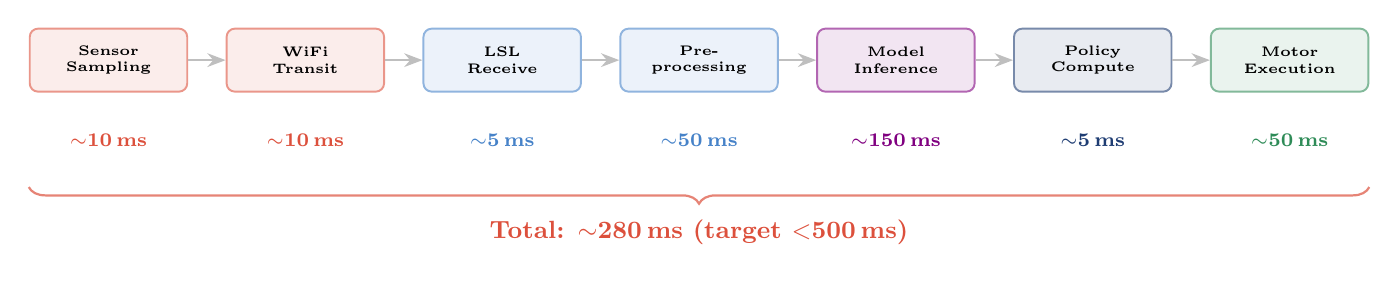
\begin{tikzpicture}[
    >=Stealth,
    stage/.style={rectangle, rounded corners=3pt, draw=#1!60, fill=#1!10, minimum width=2cm, minimum height=0.8cm, align=center, font=\tiny\bfseries, line width=0.7pt},
    time/.style={font=\scriptsize\bfseries, text=#1},
  ]

  \node[stage=accent] (s1) at (0,0) {Sensor\\Sampling};
  \node[stage=accent] (s2) at (2.5,0) {WiFi\\Transit};
  \node[stage=substratelt] (s3) at (5,0) {LSL\\Receive};
  \node[stage=substratelt] (s4) at (7.5,0) {Pre-\\processing};
  \node[stage=violet] (s5) at (10,0) {Model\\Inference};
  \node[stage=substrate] (s6) at (12.5,0) {Policy\\Compute};
  \node[stage=success] (s7) at (15,0) {Motor\\Execution};

  \foreach \s/\e in {s1/s2, s2/s3, s3/s4, s4/s5, s5/s6, s6/s7} {
    \draw[->, thick, gray!50] (\s.east) -- (\e.west);
  }

  % Timings
  \node[time=accent, below=0.4cm of s1] {$\sim$10\,ms};
  \node[time=accent, below=0.4cm of s2] {$\sim$10\,ms};
  \node[time=substratelt, below=0.4cm of s3] {$\sim$5\,ms};
  \node[time=substratelt, below=0.4cm of s4] {$\sim$50\,ms};
  \node[time=violet, below=0.4cm of s5] {$\sim$150\,ms};
  \node[time=substrate, below=0.4cm of s6] {$\sim$5\,ms};
  \node[time=success, below=0.4cm of s7] {$\sim$50\,ms};

  % Total
  \draw[decorate, decoration={brace, amplitude=6pt, mirror}, thick, accent!70]
    ([yshift=-1.2cm]s1.south west) -- ([yshift=-1.2cm]s7.south east)
    node[midway, below=8pt, font=\small\bfseries, text=accent] {Total: $\sim$280\,ms (target $<$500\,ms)};

\end{tikzpicture}
\caption{Latency budget across the data pipeline. The dominant cost is model inference.}
\label{fig:latency}
\end{figure}

\subsection{Stream Synchronisation}

All biosignal streams are transmitted via \textbf{Lab Streaming Layer (LSL)}, which provides network-level clock synchronisation across devices. Key considerations:

\begin{itemize}[leftmargin=1.5em]
  \item \textbf{Variable sample rates}: EEG at 250\,Hz, fNIRS at 10\,Hz, eye tracking at 60--120\,Hz, StretchSense at 50\,Hz, audio at 16\,kHz.
  \item The \textbf{preprocessing node} resamples all streams to a common timebase and windows them into aligned 500\,ms segments (configurable), sliding by 100\,ms for a 10\,Hz output rate.
  \item \textbf{Missing modalities}: the model should handle variable-length input or use zero-masking for absent streams, enabling graceful degradation.
\end{itemize}

\subsection{Signal Processing per Modality}

\begin{table}[H]
\centering
\caption{Preprocessing steps per biosignal modality.}
\label{tab:preprocessing}
\begin{tabularx}{\textwidth}{lX}
\toprule
\textbf{Modality} & \textbf{Preprocessing Steps} \\
\midrule
EEG & Bandpass 1--45\,Hz, notch filter 50\,Hz (mains), artifact rejection (amplitude threshold + ICA), re-referencing, epoch windowing \\
Eye Tracking & Blink removal/interpolation, fixation detection (I-VT algorithm), pupil baseline normalisation, saccade extraction \\
fNIRS & Modified Beer-Lambert Law (raw intensity $\rightarrow$ HbO/HbR concentrations), bandpass 0.01--0.2\,Hz, motion artifact correction \\
StretchSense & Calibration offset removal, first derivative for movement velocity, smoothing \\
Audio & Voice Activity Detection (VAD), pitch extraction (CREPE or pYIN), energy envelope, spectral features for prosody \\
\bottomrule
\end{tabularx}
\end{table}


% ══════════════════════════════════════════════════════════════════════════════
\section{Behaviour Design}
\label{sec:behaviour}

\subsection{State-to-Behaviour Mapping}

The behaviour policy maps the model's output state vector to robot actions. Figure~\ref{fig:behaviour-map} illustrates the mapping across key state dimensions.

\begin{figure}[H]
\centering
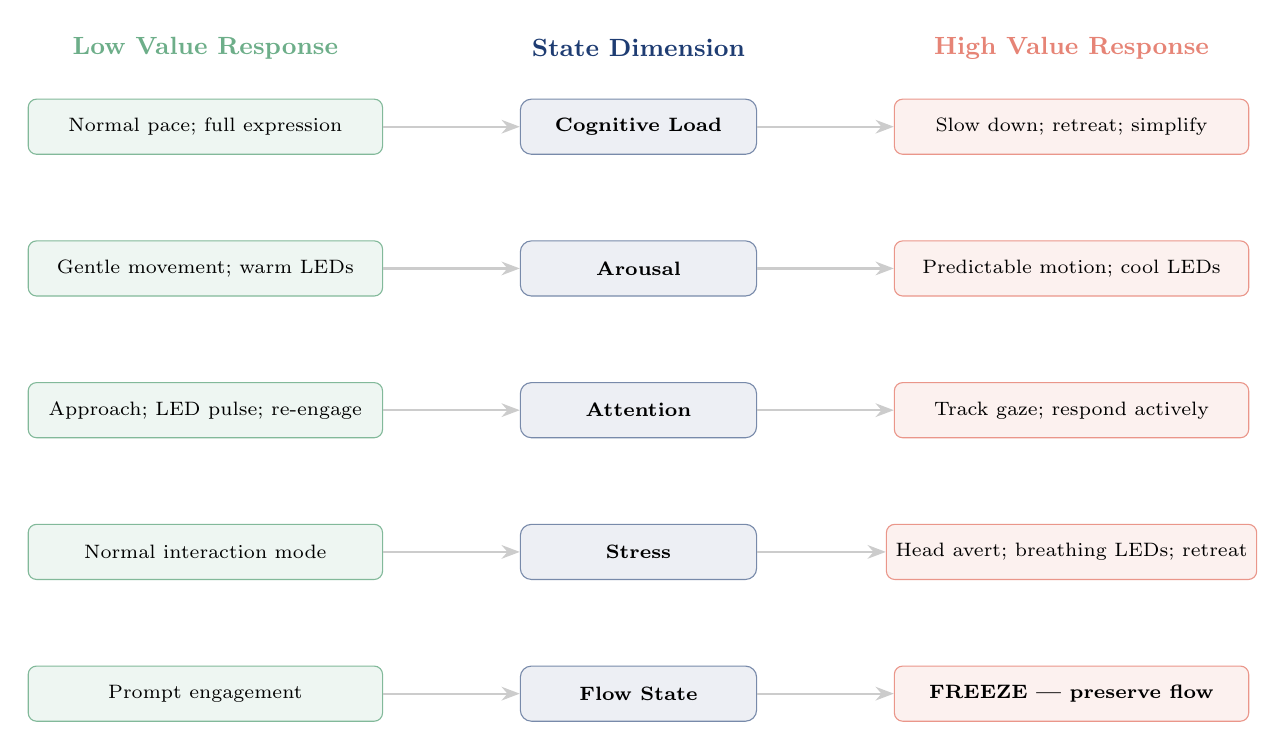
\begin{tikzpicture}[
    >=Stealth,
    state/.style={rectangle, rounded corners=4pt, draw=substrate!60, fill=substrate!8, minimum width=3cm, minimum height=0.7cm, align=center, font=\scriptsize\bfseries},
    low/.style={rectangle, rounded corners=3pt, draw=success!60, fill=success!8, minimum width=4.5cm, minimum height=0.7cm, align=center, font=\scriptsize},
    high/.style={rectangle, rounded corners=3pt, draw=accent!60, fill=accent!8, minimum width=4.5cm, minimum height=0.7cm, align=center, font=\scriptsize},
    arr/.style={->, thick, gray!40}
  ]

  % States
  \foreach \i/\name in {0/Cognitive Load, 1/Arousal, 2/Attention, 3/Stress, 4/Flow State} {
    \node[state] (s\i) at (0, -\i*1.8) {\name};
  }

  % Low responses
  \foreach \i/\resp in {%
    0/{Normal pace; full expression},
    1/{Gentle movement; warm LEDs},
    2/{Approach; LED pulse; re-engage},
    3/{Normal interaction mode},
    4/{Prompt engagement}} {
    \node[low] (l\i) at (-5.5, -\i*1.8) {\resp};
  }

  % High responses
  \foreach \i/\resp in {%
    0/{Slow down; retreat; simplify},
    1/{Predictable motion; cool LEDs},
    2/{Track gaze; respond actively},
    3/{Head avert; breathing LEDs; retreat},
    4/{\textbf{FREEZE --- preserve flow}}} {
    \node[high] (h\i) at (5.5, -\i*1.8) {\resp};
  }

  % Arrows
  \foreach \i in {0,...,4} {
    \draw[arr] (l\i.east) -- (s\i.west);
    \draw[arr] (s\i.east) -- (h\i.west);
  }

  % Headers
  \node[font=\small\bfseries, text=success!70] at (-5.5, 1.0) {Low Value Response};
  \node[font=\small\bfseries, text=substrate] at (0, 1.0) {State Dimension};
  \node[font=\small\bfseries, text=accent!70] at (5.5, 1.0) {High Value Response};

\end{tikzpicture}
\caption{Behaviour mapping: each neurobehavioural state dimension maps to distinct robot responses at low and high values. Flow state detection has highest priority and overrides all other behaviours.}
\label{fig:behaviour-map}
\end{figure}

\subsection{Behaviour Primitives}

The robot maintains a library of atomic behaviour primitives that the policy selects and blends:

\begin{lstlisting}[caption={Behaviour primitives (Python, v1 rule-based).}, label={lst:primitives}]
class BehaviourPrimitives:
    def retreat(self, distance=0.3):
        """Move base backward -- give space when overloaded."""

    def approach(self, distance=0.2):
        """Move base forward -- re-engage when attention drops."""

    def slow_breathing_led(self, period=4.0, colour=(0, 0, 80)):
        """Slow pulsing LED -- calming during high stress."""

    def alert_pulse_led(self, colour=(255, 180, 0)):
        """Quick gentle pulse -- attention bid."""

    def set_expression(self, expression: str):
        """Set face: 'neutral','attentive','calm','encouraging'"""

    def head_track(self, target_position):
        """Pan-tilt head to track human -- active engagement."""

    def head_avert(self):
        """Look away -- reduce pressure during overload."""

    def freeze(self):
        """Stop all movement -- preserve flow state."""

    def play_tone(self, tone: str):
        """Soft chime for attention bids, confirmations."""
\end{lstlisting}

\subsection{Policy Logic}

\begin{lstlisting}[caption={Priority-based behaviour policy (v1).}, label={lst:policy}]
def compute_action(state_vector, actions):
    cog_load = state_vector['cognitive_load']  # 0-1
    arousal  = state_vector['arousal']         # 0-1
    attention = state_vector['attention']      # 0-1
    stress   = state_vector['stress']          # 0-1
    flow     = state_vector['flow_state']      # 0-1

    # Priority 1: Preserve flow (override everything)
    if flow > 0.7:
        return actions.freeze()

    # Priority 2: Stress response
    if stress > 0.7:
        return actions.compose(
            actions.head_avert(),
            actions.slow_breathing_led(),
            actions.retreat(0.2),
            actions.set_expression('calm'))

    # Priority 3: Cognitive overload
    if cog_load > 0.75:
        return actions.compose(
            actions.set_expression('calm'),
            actions.retreat(0.15),
            actions.slow_breathing_led(period=5.0))

    # Priority 4: Re-engagement
    if attention < 0.3:
        return actions.compose(
            actions.approach(0.1),
            actions.alert_pulse_led(),
            actions.set_expression('attentive'))

    # Default: normal engaged interaction
    return actions.compose(
        actions.head_track(human_position),
        actions.set_expression('attentive'))
\end{lstlisting}

\begin{notebox}
Use \textbf{smooth interpolation} between behaviour states, not hard switches. Add small randomised micro-movements (gentle head sways, slow LED colour drift) to make the robot feel alive and avoid the uncanny valley of rigid state machines.
\end{notebox}


% ══════════════════════════════════════════════════════════════════════════════
\section{Build Order and Milestones}
\label{sec:milestones}

Figure~\ref{fig:gantt} shows the phased build timeline. Each phase produces a demonstrable deliverable.

\begin{figure}[H]
\centering
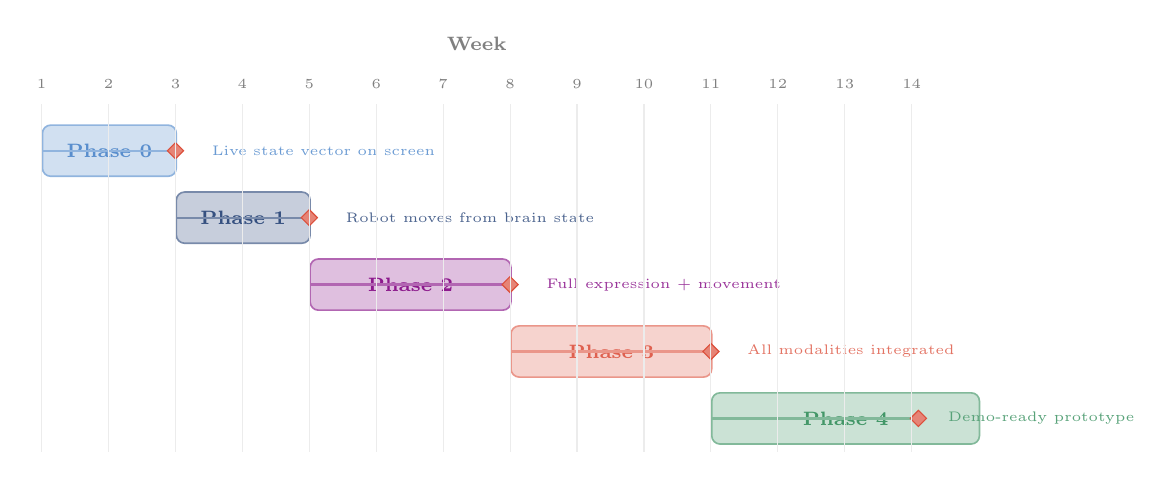
\begin{tikzpicture}[
    x=0.85cm, y=0.85cm,
    phase/.style={rectangle, rounded corners=3pt, fill=#1!25, draw=#1!60, minimum height=0.65cm, font=\scriptsize\bfseries, text=#1!90, line width=0.6pt},
    milestone/.style={diamond, fill=accent!70, draw=accent, inner sep=1.5pt, font=\tiny},
    wklbl/.style={font=\tiny, text=gray}
  ]

  % Week headers
  \foreach \w in {1,...,14} {
    \node[wklbl] at (\w, 5.5) {\w};
  }
  \node[font=\scriptsize\bfseries, text=gray] at (7.5, 6.1) {Week};

  % Phase 0: Foundations
  \node[phase=substratelt, minimum width=1.7cm, anchor=west] at (1, 4.5) {Phase 0};
  \draw[substratelt!60, thick] (1, 4.5) -- (2.9, 4.5);
  \node[milestone] at (3, 4.5) {};
  \node[font=\tiny, text=substratelt!80, anchor=west] at (3.4, 4.5) {Live state vector on screen};

  % Phase 1: Robot Base
  \node[phase=substrate, minimum width=1.7cm, anchor=west] at (3, 3.5) {Phase 1};
  \draw[substrate!60, thick] (3, 3.5) -- (4.9, 3.5);
  \node[milestone] at (5, 3.5) {};
  \node[font=\tiny, text=substrate!80, anchor=west] at (5.4, 3.5) {Robot moves from brain state};

  % Phase 2: Expressive Head
  \node[phase=violet, minimum width=2.55cm, anchor=west] at (5, 2.5) {Phase 2};
  \draw[violet!60, thick] (5, 2.5) -- (7.9, 2.5);
  \node[milestone] at (8, 2.5) {};
  \node[font=\tiny, text=violet!80, anchor=west] at (8.4, 2.5) {Full expression + movement};

  % Phase 3: Multi-Modal
  \node[phase=accent, minimum width=2.55cm, anchor=west] at (8, 1.5) {Phase 3};
  \draw[accent!60, thick] (8, 1.5) -- (10.9, 1.5);
  \node[milestone] at (11, 1.5) {};
  \node[font=\tiny, text=accent!80, anchor=west] at (11.4, 1.5) {All modalities integrated};

  % Phase 4: Polish
  \node[phase=success, minimum width=3.4cm, anchor=west] at (11, 0.5) {Phase 4};
  \draw[success!60, thick] (11, 0.5) -- (14, 0.5);
  \node[milestone] at (14.1, 0.5) {};
  \node[font=\tiny, text=success!80, anchor=west] at (14.4, 0.5) {Demo-ready prototype};

  % Grid lines
  \foreach \w in {1,...,14} {
    \draw[gray!15] (\w, 0) -- (\w, 5.2);
  }

\end{tikzpicture}
\caption{Build timeline across 14 weeks with five phases. Each diamond marks a demonstrable milestone.}
\label{fig:gantt}
\end{figure}

\subsection{Phase 0: Software Foundations (Weeks 1--2)}

\begin{milestonebox}[title={Deliverable: Human wears EEG, state vector updates live on screen}]
\begin{itemize}[leftmargin=1.5em, nosep]
  \item Set up ROS2 Humble on Ubuntu 22.04 (development laptop)
  \item Write \texttt{lsl\_receiver\_node}---connect to one real LSL stream (e.g. EEG headset)
  \item Write \texttt{preprocessing\_node}---basic bandpass filter, publish processed data
  \item Write \texttt{inference\_node}---load foundation model in PyTorch, run inference on windowed data
  \item Verify end-to-end: EEG $\rightarrow$ LSL $\rightarrow$ preprocessing $\rightarrow$ model $\rightarrow$ state vector on terminal
  \item Define custom ROS2 message types (\texttt{NeuroBehaviouralState.msg})
\end{itemize}
\end{milestonebox}

\subsection{Phase 1: Robot Base (Weeks 3--4)}

\begin{milestonebox}[title={Deliverable: Robot physically moves in response to human brain state}]
\begin{itemize}[leftmargin=1.5em, nosep]
  \item Acquire and bring up TurtleBot4 Lite in ROS2
  \item Verify \texttt{/cmd\_vel} control (keyboard teleop first)
  \item Write \texttt{behaviour\_policy\_node}---map state vector to approach/retreat
  \item Connect full loop: human state $\rightarrow$ robot movement
  \item Set up Jetson Orin NX, flash JetPack, install ROS2 + PyTorch
  \item Migrate all nodes from laptop to Jetson
\end{itemize}
\end{milestonebox}

\subsection{Phase 2: Expressive Head (Weeks 5--7)}

\begin{milestonebox}[title={Deliverable: Robot moves, looks at you, changes expression and LEDs based on state}]
\begin{itemize}[leftmargin=1.5em, nosep]
  \item Design and 3D-print head housing
  \item Mount Dynamixel pan-tilt + round display
  \item Write \texttt{face\_expression\_node}---animated eyes (pygame or lightweight OpenGL)
  \item Write \texttt{head\_control\_node}---pan-tilt tracking
  \item Mount LED ring, write \texttt{led\_node}
  \item Add speaker + amplifier, write \texttt{audio\_node}
  \item Expand behaviour policy to use all output channels
\end{itemize}
\end{milestonebox}

\subsection{Phase 3: Multi-Modal Input (Weeks 8--10)}

\begin{milestonebox}[title={Deliverable: Full multimodal input, richer state vector, nuanced behaviour}]
\begin{itemize}[leftmargin=1.5em, nosep]
  \item Add eye tracking, fNIRS, StretchSense, and microphone to LSL pipeline
  \item Update \texttt{preprocessing\_node} for each modality
  \item Handle variable sample rates: resampling and temporal alignment
  \item Retune windowing parameters
  \item Validate state vector quality with all streams active
\end{itemize}
\end{milestonebox}

\subsection{Phase 4: Polish and Optimise (Weeks 11--14)}

\begin{milestonebox}[title={Deliverable: Robust, low-latency, demo-ready prototype}]
\begin{itemize}[leftmargin=1.5em, nosep]
  \item Convert model to TensorRT, benchmark on Jetson
  \item Profile and optimise full pipeline latency
  \item Add \texttt{rosbag2} recording for experiment logging
  \item Add Foxglove Studio dashboard for live monitoring
  \item Tune behaviour policy with real users (iterative)
  \item Safety features: e-stop button, collision avoidance
  \item Design and print final housing
\end{itemize}
\end{milestonebox}


% ══════════════════════════════════════════════════════════════════════════════
\section{Risks and Mitigations}
\label{sec:risks}

\begin{figure}[H]
\centering
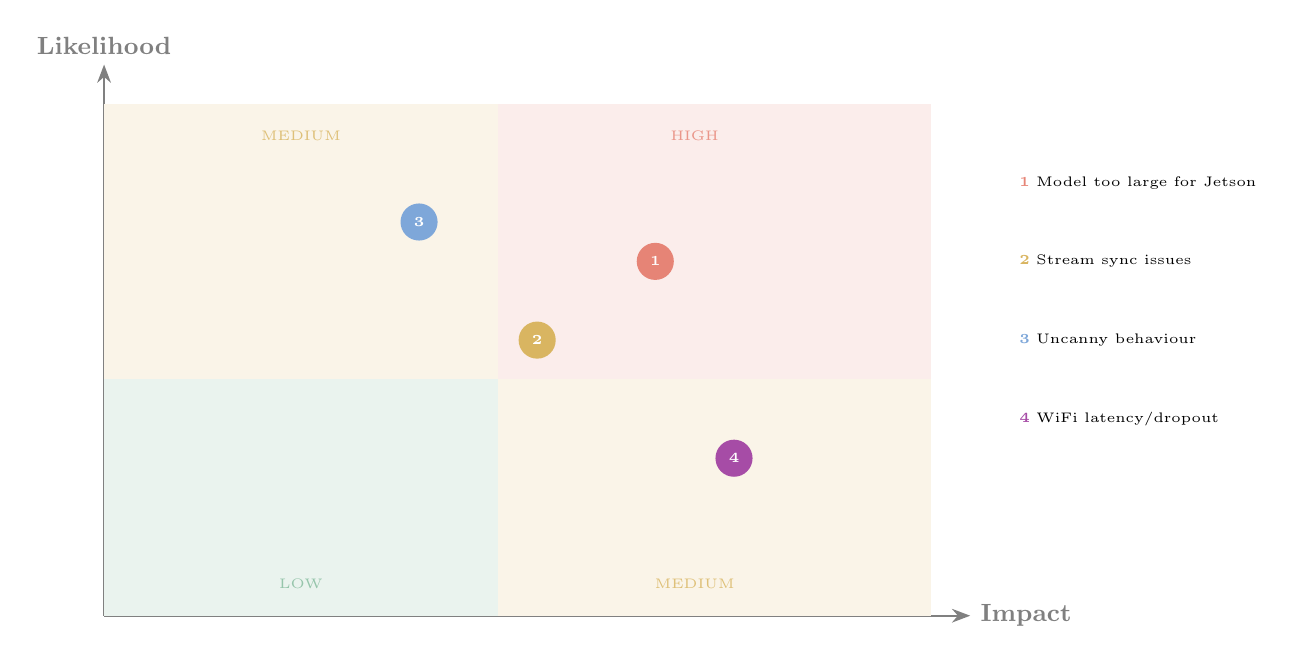
\begin{tikzpicture}[
    x=1cm, y=1cm,
    >=Stealth
  ]

  % Axes
  \draw[->, thick, gray] (0,0) -- (11,0) node[right, font=\small\bfseries, text=gray] {Impact};
  \draw[->, thick, gray] (0,0) -- (0,7) node[above, font=\small\bfseries, text=gray] {Likelihood};

  % Grid
  \foreach \x in {2,4,6,8,10} {
    \draw[gray!15] (\x,0) -- (\x,6.5);
  }
  \foreach \y in {1,...,6} {
    \draw[gray!15] (0,\y) -- (10.5,\y);
  }

  % Risk zones
  \fill[success!10] (0,0) rectangle (5,3);
  \fill[warn!10] (5,0) rectangle (10.5,3);
  \fill[warn!10] (0,3) rectangle (5,6.5);
  \fill[accent!10] (5,3) rectangle (10.5,6.5);

  \node[font=\tiny, text=success!50] at (2.5, 0.4) {LOW};
  \node[font=\tiny, text=warn!60] at (7.5, 0.4) {MEDIUM};
  \node[font=\tiny, text=warn!60] at (2.5, 6.1) {MEDIUM};
  \node[font=\tiny, text=accent!60] at (7.5, 6.1) {HIGH};

  % Risk points
  \node[circle, fill=accent!70, text=white, font=\tiny\bfseries, inner sep=3pt] (r1) at (7, 4.5) {1};
  \node[circle, fill=warn!70, text=white, font=\tiny\bfseries, inner sep=3pt] (r2) at (5.5, 3.5) {2};
  \node[circle, fill=substratelt!70, text=white, font=\tiny\bfseries, inner sep=3pt] (r3) at (4, 5) {3};
  \node[circle, fill=violet!70, text=white, font=\tiny\bfseries, inner sep=3pt] (r4) at (8, 2) {4};

  % Legend
  \node[font=\tiny, anchor=west] at (11.5, 5.5) {\textcolor{accent!70}{\textbf{1}} Model too large for Jetson};
  \node[font=\tiny, anchor=west] at (11.5, 4.5) {\textcolor{warn!70}{\textbf{2}} Stream sync issues};
  \node[font=\tiny, anchor=west] at (11.5, 3.5) {\textcolor{substratelt!70}{\textbf{3}} Uncanny behaviour};
  \node[font=\tiny, anchor=west] at (11.5, 2.5) {\textcolor{violet!70}{\textbf{4}} WiFi latency/dropout};

\end{tikzpicture}
\caption{Risk matrix. Numbered risks are detailed in the mitigations below.}
\label{fig:risk-matrix}
\end{figure}

\begin{riskbox}[title={\faExclamationTriangle\ Risk 1: Model Too Large for Jetson}]
\textbf{Mitigation}: Design the inference node to support both local and remote backends from day one. Start with server offload (WiFi + gRPC), optimise with TensorRT/quantisation, and migrate to Jetson once the model fits. A gRPC round-trip on local 5\,GHz WiFi adds only $\sim$20--50\,ms.
\end{riskbox}

\begin{riskbox}[title={\faExclamationTriangle\ Risk 2: Multi-Stream Synchronisation}]
\textbf{Mitigation}: LSL handles clock sync well, but test with all streams simultaneously early in Phase~3. Variable sample rates (EEG 250\,Hz, fNIRS 10\,Hz, eye tracking 60--120\,Hz) require explicit resampling and temporal alignment in the preprocessing node. Build alignment unit tests before integrating.
\end{riskbox}

\begin{riskbox}[title={\faExclamationTriangle\ Risk 3: Uncanny / Robotic Behaviour}]
\textbf{Mitigation}: Use smooth interpolation between behaviour states, not hard threshold switches. Add randomised micro-movements (small head sways, gentle LED colour drift) to create liveliness. Tune transition speeds empirically with real users---budget significant time in Phase~4 for this.
\end{riskbox}

\begin{riskbox}[title={\faExclamationTriangle\ Risk 4: WiFi Latency or Dropout}]
\textbf{Mitigation}: Use a \textbf{dedicated 5\,GHz WiFi router} (not shared network) travelling with the setup. Consider a USB WiFi dongle for the most critical low-latency stream (e.g. EEG) if standard WiFi proves unreliable. Implement a brief state-hold buffer so the robot maintains its last known state during transient dropouts.
\end{riskbox}


% ══════════════════════════════════════════════════════════════════════════════
\section{Data Clarification}
\label{sec:clarification}

\begin{riskbox}[title={\faExclamationTriangle\ Important: Input Modality Mismatch}]
The foundation model specification states that inference takes \textbf{EEG, ECG, and IMU} as inputs. However, the recorded data description explicitly states \textbf{no ECG} and \textbf{no IMU} (StretchSense measures deformation, not inertial data) in either recording configuration.

\medskip\noindent
This must be resolved before wiring the pipeline:
\begin{itemize}[leftmargin=1.5em, nosep]
  \item If the model genuinely requires ECG and IMU: source a wearable ECG (e.g. Polar H10, BLE + LSL bridge) and IMU (e.g. Movella DOT) for the human to wear during operation.
  \item If the model was trained on the recorded modalities (EEG, eye tracking, fNIRS, StretchSense, audio): update the inference specification to match.
\end{itemize}
\end{riskbox}


% ══════════════════════════════════════════════════════════════════════════════
\section{Future Directions}
\label{sec:future}

\begin{enumerate}[leftmargin=1.5em]
  \item \textbf{Learned Behaviour Policy (Phase~5)}: Replace the rule-based policy with a reinforcement learning agent. Use recorded \texttt{rosbag2} data and human feedback to train the policy. The foundation model's state embeddings become the RL observation space.

  \item \textbf{Manipulation}: Add a single robot arm (e.g. Trossen PincherX 100) for handing objects, pointing, or gestural communication.

  \item \textbf{Multi-Person Interaction}: Extend the system to read biosignals from multiple participants simultaneously and manage group interaction dynamics.

  \item \textbf{Longitudinal Adaptation}: Store state history per individual and adapt the robot's baseline behaviour over repeated interactions.

  \item \textbf{Clinical Applications}: Deploy the platform in therapeutic contexts (e.g. stress management, attention training, cognitive rehabilitation) with clinician-designed behaviour protocols.
\end{enumerate}


% ══════════════════════════════════════════════════════════════════════════════
\appendix
\section{Communication Topology}
\label{app:topology}

\begin{figure}[H]
\centering
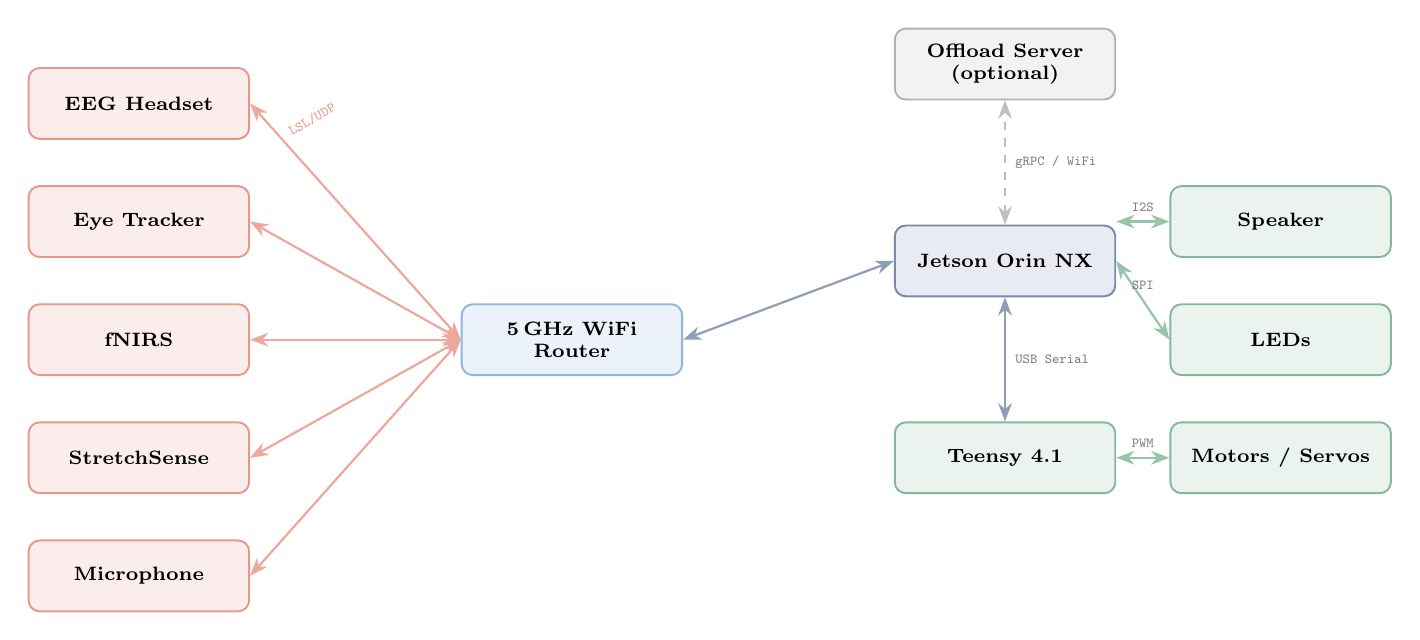
\begin{tikzpicture}[
    >=Stealth,
    device/.style={rectangle, rounded corners=4pt, draw=#1!60, fill=#1!10, minimum width=2.8cm, minimum height=0.9cm, align=center, font=\scriptsize\bfseries, line width=0.7pt},
    link/.style={<->, thick, #1!50}
  ]

  % Devices
  \node[device=accent] (eeg) at (0, 4) {EEG Headset};
  \node[device=accent] (eye) at (0, 2.5) {Eye Tracker};
  \node[device=accent] (fnirs) at (0, 1) {fNIRS};
  \node[device=accent] (stretch) at (0, -0.5) {StretchSense};
  \node[device=accent] (mic) at (0, -2) {Microphone};

  \node[device=substratelt] (router) at (5.5, 1) {5\,GHz WiFi\\Router};

  \node[device=substrate] (jetson) at (11, 2) {Jetson Orin NX};
  \node[device=success] (teensy) at (11, -0.5) {Teensy 4.1};
  \node[device=success] (motors) at (14.5, -0.5) {Motors / Servos};
  \node[device=success] (leds) at (14.5, 1) {LEDs};
  \node[device=success] (speaker) at (14.5, 2.5) {Speaker};
  \node[device=gray] (server) at (11, 4.5) {Offload Server\\(optional)};

  % Links
  \foreach \src in {eeg, eye, fnirs, stretch, mic} {
    \draw[link=accent] (\src.east) -- (router.west);
  }
  \draw[link=substrate] (router.east) -- (jetson.west);
  \draw[link=substrate] (jetson.south) -- (teensy.north) node[midway, right, font=\tiny\ttfamily, text=gray] {USB Serial};
  \draw[link=success] (teensy.east) -- (motors.west) node[midway, above, font=\tiny\ttfamily, text=gray] {PWM};
  \draw[link=success] (jetson.east) -- (leds.west) node[midway, above, font=\tiny\ttfamily, text=gray] {SPI};
  \draw[link=success] (jetson.east) ++ (0,0.5) -- (speaker.west) node[midway, above, font=\tiny\ttfamily, text=gray] {I2S};
  \draw[link=gray, dashed] (jetson.north) -- (server.south) node[midway, right, font=\tiny\ttfamily, text=gray] {gRPC / WiFi};

  % Protocol labels on WiFi links
  \node[font=\tiny\ttfamily, text=accent!60, rotate=30] at (2.2, 3.8) {LSL/UDP};

\end{tikzpicture}
\caption{Full communication topology showing all physical and network links.}
\label{fig:topology}
\end{figure}


% ══════════════════════════════════════════════════════════════════════════════
\vfill
\begin{center}
\textcolor{substrate}{\rule{0.6\textwidth}{0.4pt}}\\[0.3cm]
{\small\textcolor{substrate}{\textbf{Substrate House}} \textperiodcentered\ London \textperiodcentered\ 2026}\\[0.2cm]
{\footnotesize\textcolor{gray}{Document generated as part of the Neurobehavioural Adaptive Robot project.}}
\end{center}

\end{document}
